\section{Introduction}
\noindent Video inpainting aims to recover the missing contents of given videos, which can assist lots of practical applications, e.g., video restoration and augmented reality. Compared with image inpainting, video inpainting is much more challenging due to extra time dimension. It requires not only reasonable spatial structures but also stable temporal consistency. Specifically, directly applying 2D image inpainting algorithm \cite{yu2018free,Xiong_2019_CVPR} to individual frames is a sub-optimal choice, due to serious artificial effect, flickers and jitters. 

To exploit complementary neighboring information across frames, traditional patch-based methods \cite{patwardhan2007video,wexler2004space,newson2014video} recurrently copy the similar patches from unmasked regions and past them to the missing regions. 
\begin{figure}[t]
	\centering
	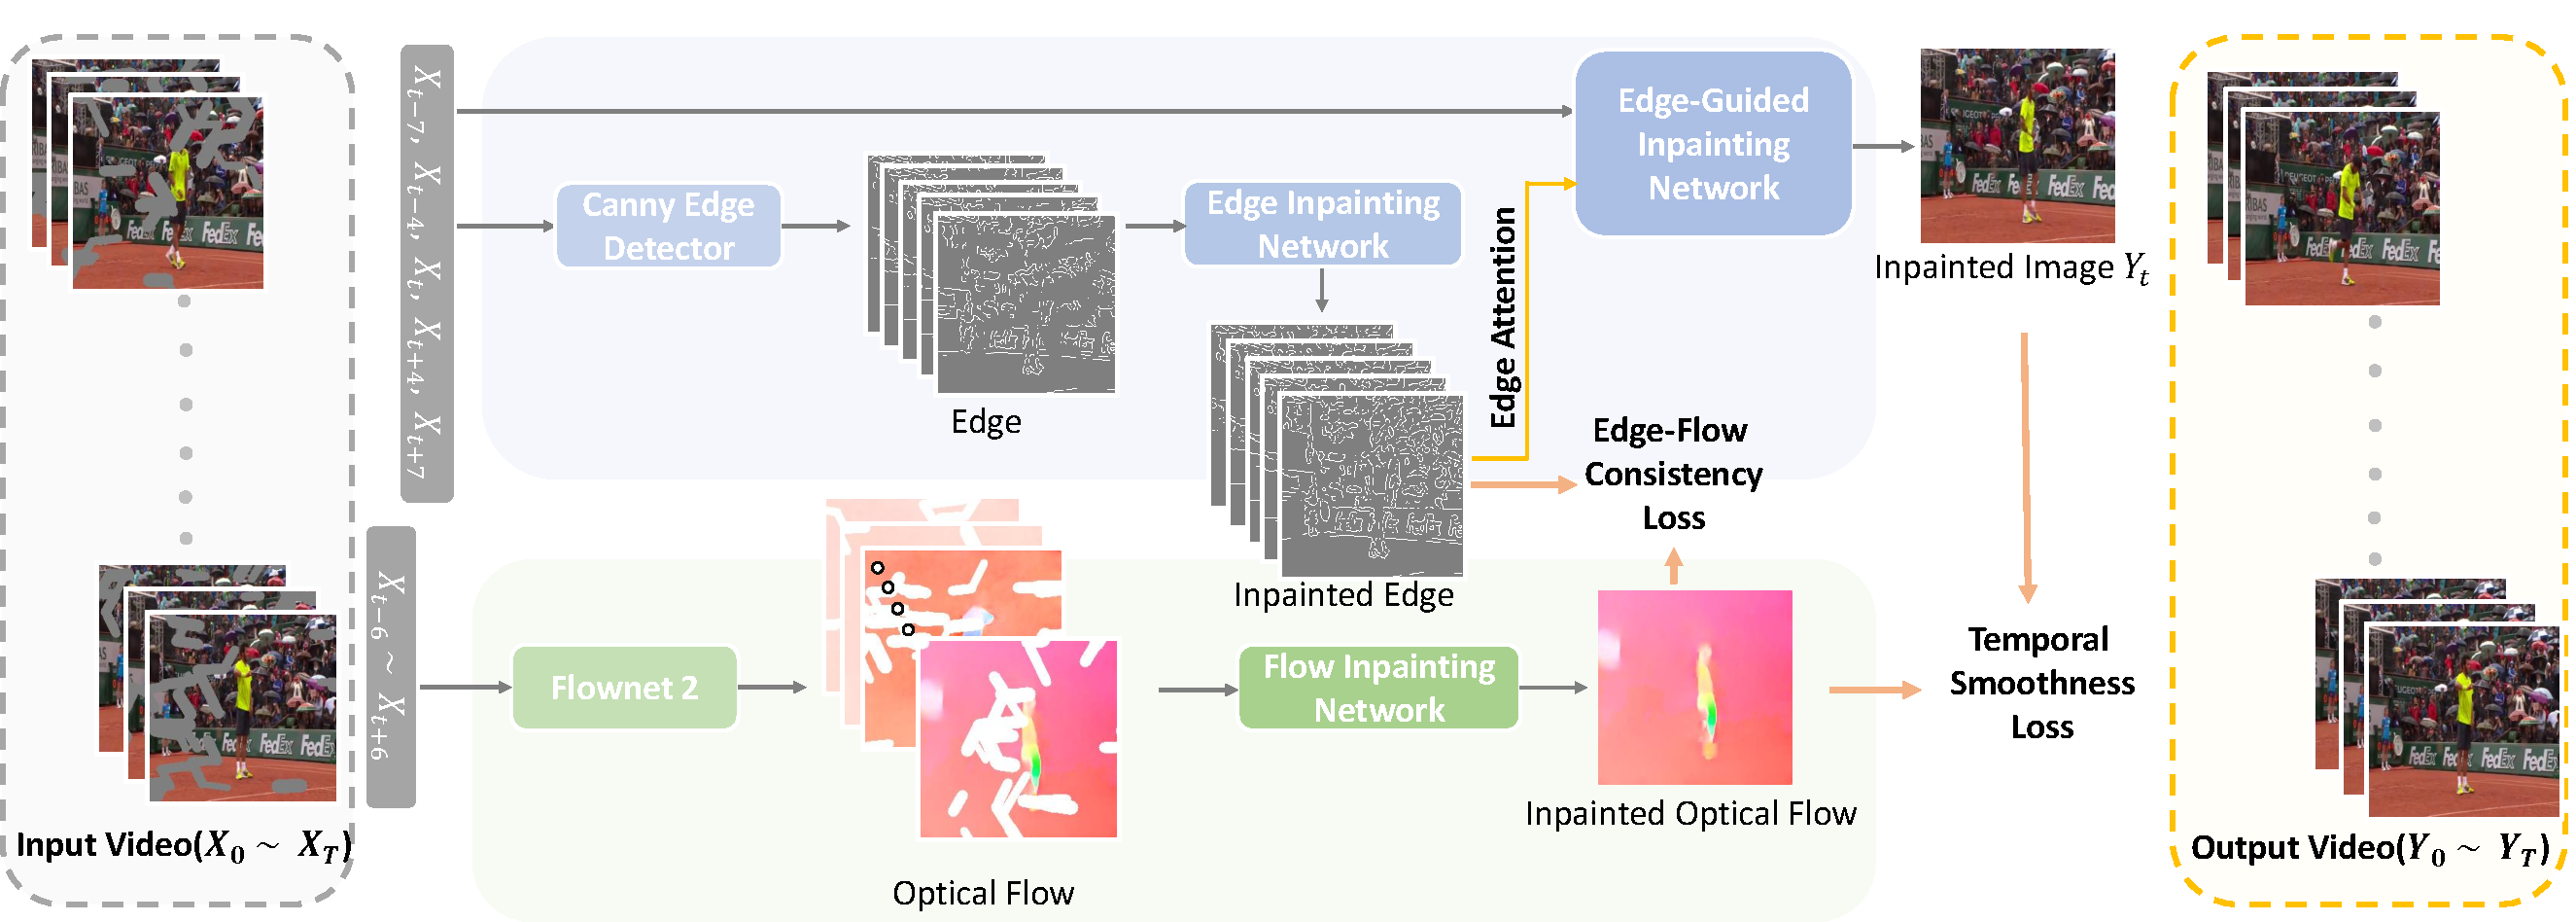
\includegraphics[width=1.0\columnwidth]{zong} % Reduce the figure size so that it is slightly narrower than the column. Don't use precise values for figure width.This setup will avoid overfull boxes. 
	\caption{The overall pipeline of our method. The ENet first completes the missing edge across frames. Then, under the guidance of auxiliary edge, STI can produce structure-preserved inpainting frame. Moreover, the FNet is designed to predict missing optical flow, which provides temporally consistency to the final result.}
	\label{zong}
\end{figure}
This kind of methods depends on a strong hypothesis that the missing content have precisely appeared in neighboring frames, which limits their generalization.
Recently, deep-learning based methods achieve state-of-the-art performance by treating a video as volume.
They utilize the CNNs, e.g., 3D convolution operation \cite{wang2019video}, to predict missing content with smooth motion, which is learned from training data.
Among these methods, optical flow is commonly used to temporally smooth the inpainted contents \cite{Xu_2019_CVPR,Kim_2019_CVPR,Kim_2019_CVPR1} by aggregating the contextual information from neighboring frames.
However, the auxiliary motion compensation brought by optical flow lacks detailed structural clues,~\emph{e.g.}~the inner textures of objects are usually missed in flow field, leading to deficient structure rationality.
Thus, how to obtain fine-detailed inpainting video remains an open problem.





\begin{figure*}[t]
	\centering
	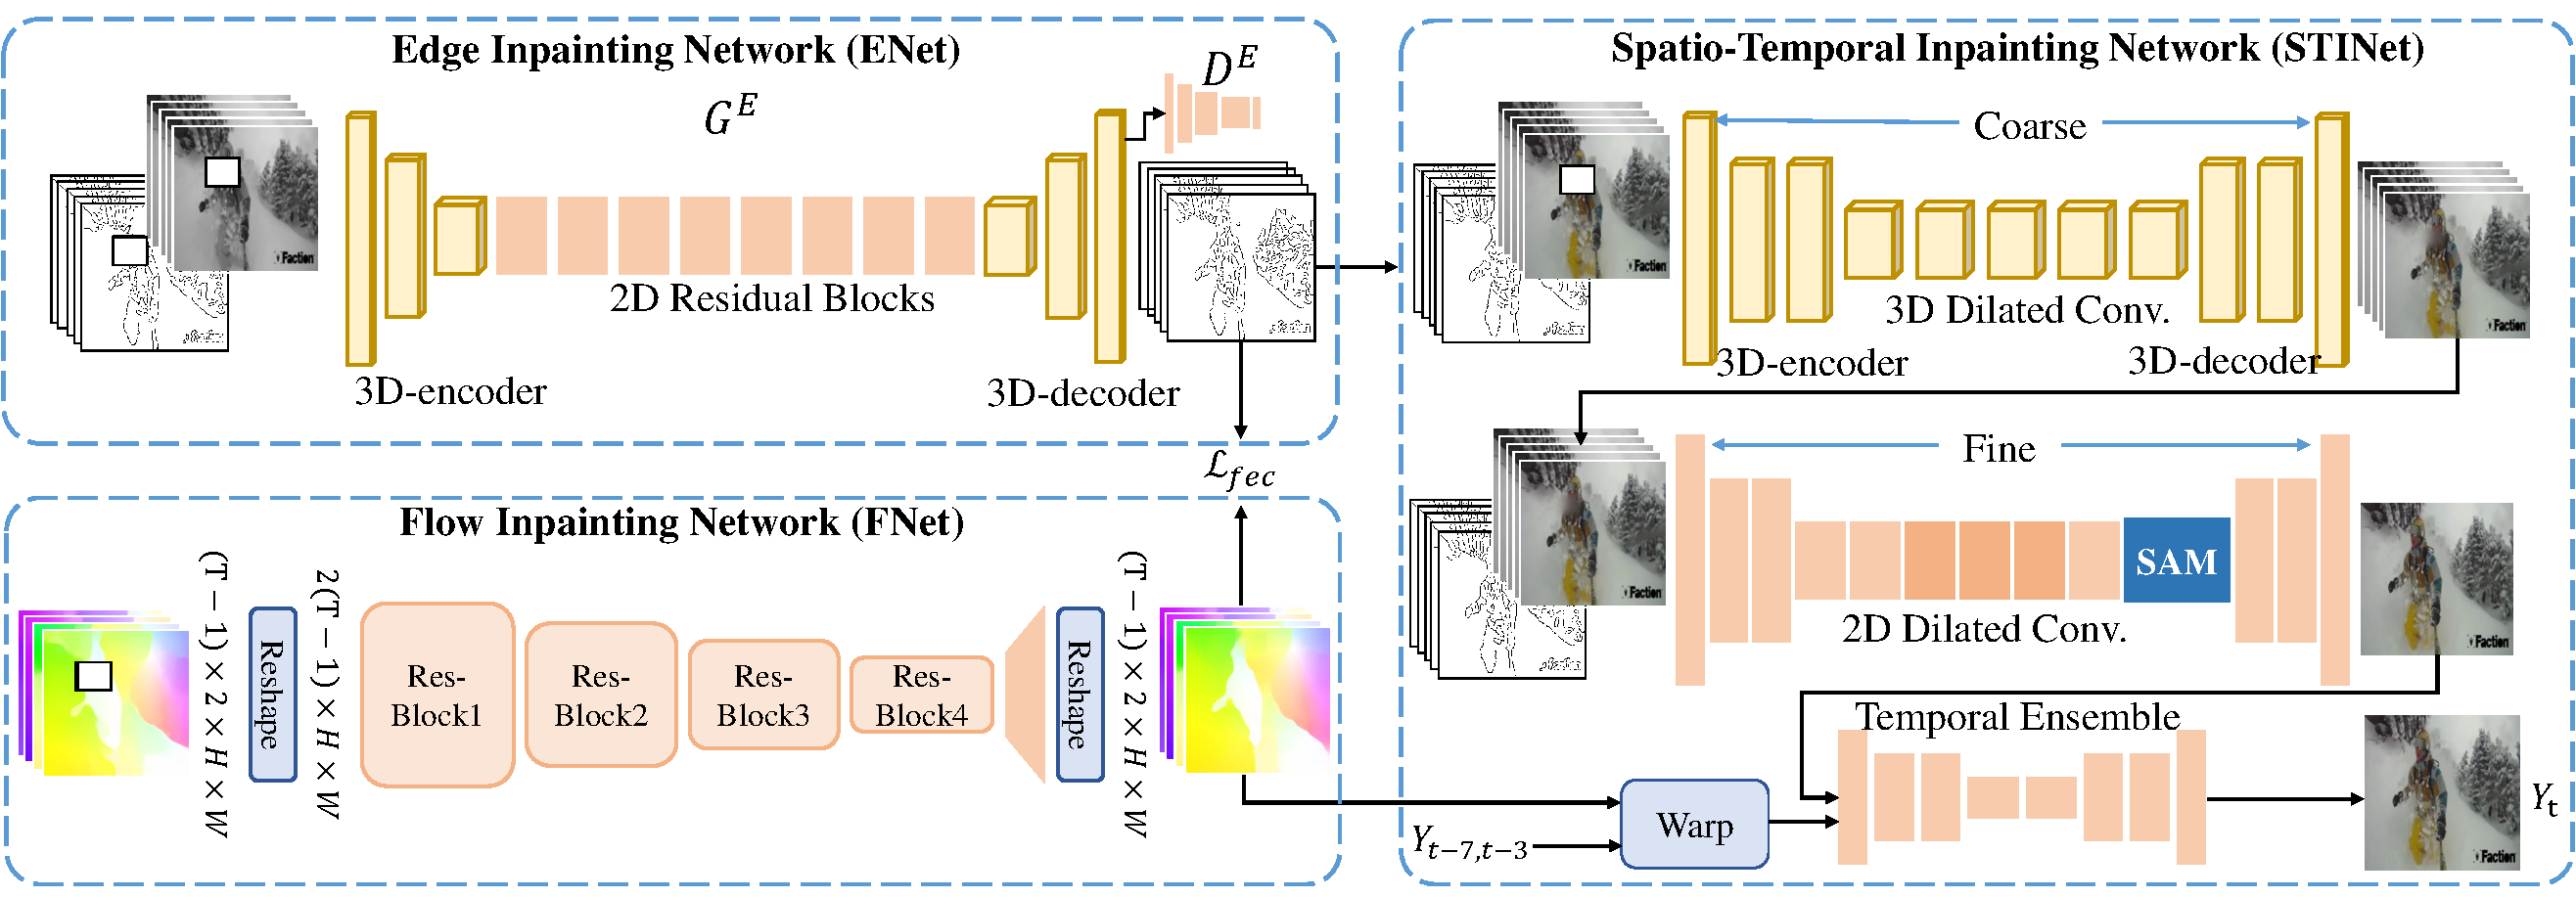
\includegraphics[width=2.0\columnwidth]{sti} % Reduce the figure size so that it is slightly narrower than the column. Don't use precise values for figure width.This setup will avoid overfull boxes. 
	\caption{The detailed architecture of ENet and STI. ENet adopts an encoder-decoder architectures with heterogeneous receptive field. STI is followed to inpaint the frames in a coarse-to-fine manner. To save space, all the input masks are omitted.}
	
	%	. . FNet uses the Resnet101 as backbone, followed by a decoder. STI . In FNet, $T$ is the number of input frames, and channel $2$ denotes the motion along $x$ and $y$ axis. }
	\label{fig:stiNet}
\end{figure*}
In this paper, we present a novel structure-oriented video inpainting network (SOVI) that can collect and refine the structure information to improve the inpainting results. As shown in Fig.~\ref{zong}, our method consists of three modules, which are respectively the Edge Inpainting Network (ENet), Flow Inpainting Network (FNet), and Spatio-Temporal Inpainting Network (STINet).
Given frames with missing pixels, ENet first completes the edge maps that indicate the detailed structure information. Then, under the guidance of completed edge, STI is developed to fill the missing colors and textures in a coarse-to-fine manner.
Specifically, a structure attention module is designed to capture the latent spatial relevance between video contents and structure edges.
Such a spatial relevance clues is easier to be absorbed by STI than original edge maps, which helps STI to generate fine-detailed inpainted frames.
Besides, the developed FNet can predict the missing optical flow, which provides auxiliary motion knowledge. Explicitly, a flow-edge consistency constraint and a temporal ensemble module are utilized to smoothen the edge maps and final inpainted frames, based on the motion tendency. Consequently, the inpainted frames by our method are not only detail-preserved but also temporal consistent.
%by simultaneously exploring optical flow and , to eliminate temporal flickers and enhance spatial detail. 
%  and FNet  and optical flow,  knowledge and motion tendency.
%according to learned structure knowledge and motion tendency from the training data,
%Instead of separate training, these two modules are
%This results in both edge-enhanced optical flow and temporally smooth edge. 
%Specifically, a structure enhancement mechanism is developed to extract and refine the structural clues in the completed edge and encode them into the STI.
% the optical flow is used by propagating complementary pixels from neighboring frames to current frame to alleviate artificial flickers and jitters.
Experiments on YouTubeVOS and DAVIS datasets show that the proposed method obtains new state-of-the-art performance with low time consumption, which demonstrates its superiority.
Our contributions can be summarized as follows.
\begin{itemize}
	\item A novel structure-oriented video inpainting method is proposed, which can generate structural reasonable and temporal coherent inpainted frames.
	
	\item We introduce an edge inpainting network to predict the missing edges. Further, a novel structure attention module is designed to capture the spatial relevance between video contents and structure edges, which is then embedded into the video inpainting. %With edge collection and structure embedding, we demonstrate the significance of detailed structure in video inpainting. 
	%to structure information is well represented and encoded in video inpainting via . 
	\item A flow-guided warping and temporal ensemble module are developed to enhance temporal consistency.
	%	Optical flow is used to enhance temporal consistency, which 
	
	
	%	We propose a novel structure- for video inpainting, by simultaneously exploring optical flow and structural clues to eliminate temporal flickers and enhance structure detail. 
	%	 A flow-edge consistency loss is developed to associate the optical flow and structure edges, which can boost each other.
	%	\item  a structure enhancement mechanism is  designed, which can promote the video inpainting.	
	
\end{itemize}





\section{Related Work}